\documentclass[tikz,border=15pt]{standalone}
\usepackage{tikz}
\usepackage{amsmath}
\usetikzlibrary{arrows.meta,positioning,shapes}

\begin{document}
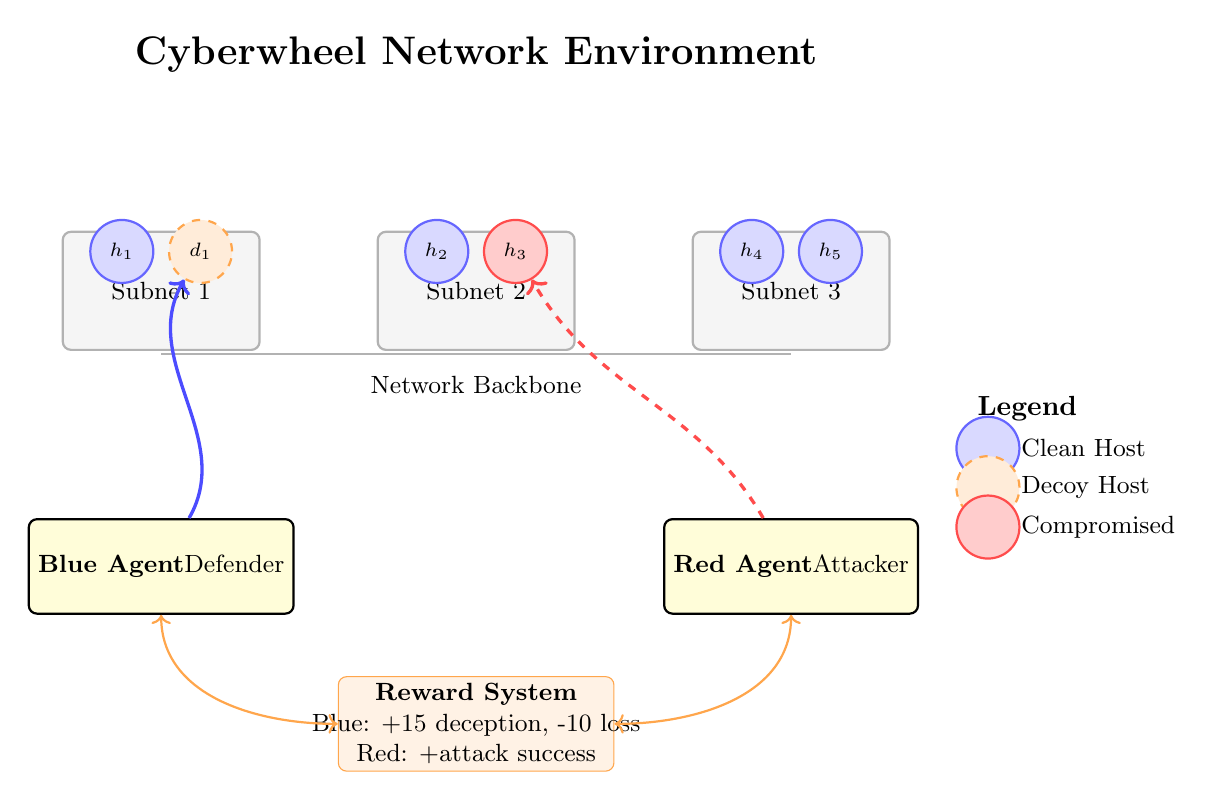
\begin{tikzpicture}[
    host/.style={circle, draw=blue!60, fill=blue!15, minimum size=8mm, font=\scriptsize, thick},
    decoy/.style={circle, draw=orange!70, fill=orange!15, minimum size=8mm, font=\scriptsize, thick, dashed},
    compromised/.style={circle, draw=red!70, fill=red!20, minimum size=8mm, font=\scriptsize, thick},
    subnet/.style={rectangle, draw=gray!60, fill=gray!8, minimum width=25mm, minimum height=15mm, font=\small, thick, rounded corners=3pt},
    agent/.style={rectangle, draw=black, fill=yellow!15, minimum width=20mm, minimum height=12mm, font=\small, thick, rounded corners=3pt}
]

% Title - plenty of space above
\node[font=\Large\bfseries] at (0, 7) {Cyberwheel Network Environment};

% Network subnets - well separated horizontally  
\node[subnet] (subnet1) at (-4, 4) {Subnet 1};
\node[subnet] (subnet2) at (0, 4) {Subnet 2};  
\node[subnet] (subnet3) at (4, 4) {Subnet 3};

% Hosts - positioned clearly within each subnet
\node[host] (h1) at (-4.5, 4.5) {$h_1$};
\node[decoy] (d1) at (-3.5, 4.5) {$d_1$};

\node[host] (h2) at (-0.5, 4.5) {$h_2$};
\node[compromised] (h3) at (0.5, 4.5) {$h_3$};

\node[host] (h4) at (3.5, 4.5) {$h_4$};
\node[host] (h5) at (4.5, 4.5) {$h_5$};

% Network backbone - clear separation from subnets
\draw[gray!60, thick] (-4, 3.2) -- (0, 3.2) -- (4, 3.2);
\node[font=\small] at (0, 2.8) {Network Backbone};

% Agents - lots of vertical space from network
\node[agent] (blue) at (-4, 0.5) {\textbf{Blue Agent}\\Defender};
\node[agent] (red) at (4, 0.5) {\textbf{Red Agent}\\Attacker};

% Simple arrows - no text overlap
\draw[->, very thick, blue!70] (blue) to[out=60, in=240] (d1);
\draw[->, very thick, red!70, dashed] (red) to[out=120, in=300] (h3);

% Legend - positioned far to avoid overlap
\node at (7, 2.5) {\textbf{Legend}};
\node[host] at (6.5, 2) {}; \node[right, font=\small] at (6.8, 2) {Clean Host};
\node[decoy] at (6.5, 1.5) {}; \node[right, font=\small] at (6.8, 1.5) {Decoy Host};
\node[compromised] at (6.5, 1) {}; \node[right, font=\small] at (6.8, 1) {Compromised};

% Reward system - bottom, well separated
\node[rectangle, draw=orange!70, fill=orange!10, minimum width=35mm, minimum height=12mm, rounded corners=3pt] at (0, -1.5) (reward) {};
\node[font=\small, align=center] at (reward.center) {\textbf{Reward System}\\Blue: +15 deception, -10 loss\\Red: +attack success};

% Connection lines to reward - clean
\draw[<->, orange!70, thick] (blue) to[out=270, in=180] (reward);
\draw[<->, orange!70, thick] (red) to[out=270, in=0] (reward);

\end{tikzpicture}
\end{document}